%----------------------------------------------------------------------------
\chapter{Áttekintés}
%----------------------------------------------------------------------------
%Mit csinál
%Mire jó (szerkesztés, finomítás?, import? új objektumok...)
%(technológia nélkül)


A cél egy olyan metamodell elkészítése, ami segítségével lehetséges részleges modelleket készíteni. Ehhez olyan vizuális szerkesztőfelület társul, ami megkönnyíti ezt a folyamatot. Ahhoz, hogy ez generikusan működjön egy olyan modell szükséges, aminek segítségével a lehető legtöbb egyéb modell kifejezhető. Így ez a metamodell tartalmazni fog objektumokat, attribútumokat és az ezek közti kapcsolatot kifejező referenciákat. Ezen felül a részlegesség kifejezésére minden ilyen elemhez lehetséges rendelni \textit{May}, \textit{Var} vagy \textit{Abs} részlegességet. Magához a modellhez pedig \textit{OW} partiality-t lehet rendelni.
A kapcsolódó editor képes részleges modellt létrehozni és manipulálni. Lehetőséget ad új objektumok, attribútumok, referenciák létrehozására. Ezen elemekhez a már fent említett részlegességek rendelhetők. A szerkesztő a részlegességek feloldására, tehát finomításra is biztosít eszközöket.



\begin{figure}[!ht]
	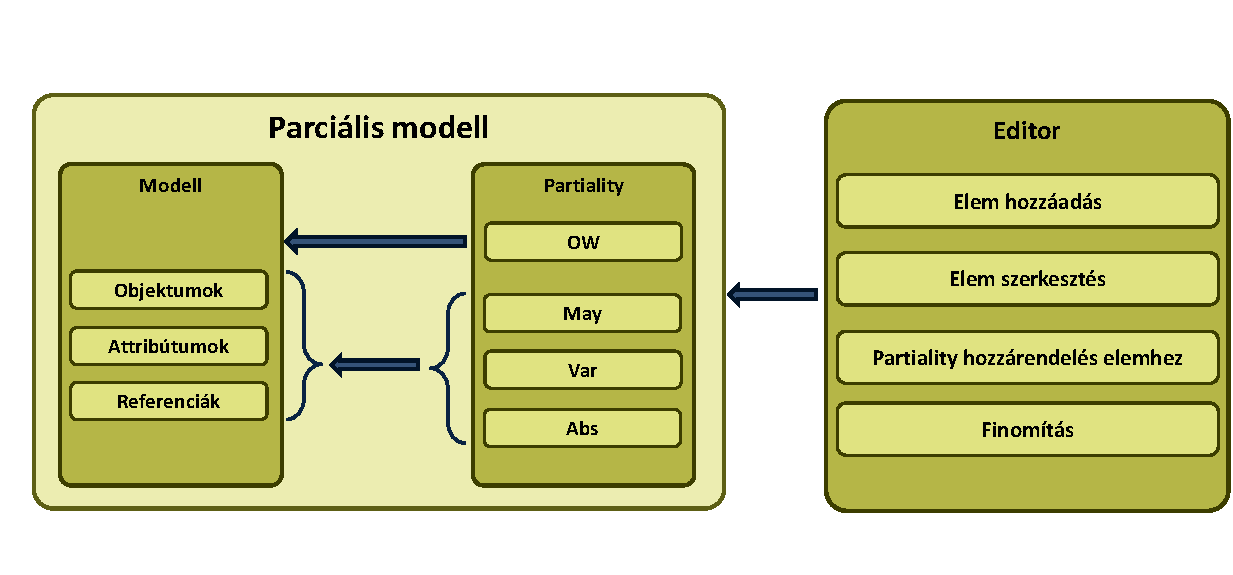
\includegraphics[width=150mm]{figures/overview.pdf}
	\caption{Áttekintő} 
\end{figure}

